%  LaTeX support: latex@mdpi.com 
%  For support, please attach all files needed for compiling as well as the log file, and specify your operating system, LaTeX version, and LaTeX editor.

%=================================================================
\documentclass[forecasting,article,submit,pdftex,moreauthors]{Definitions/mdpi}
%\documentclass[preprints,article,submit,pdftex,moreauthors]{Definitions/mdpi}
% For posting an early version of this manuscript as a preprint, you may use "preprints" as the journal. Changing "submit" to "accept" before posting will remove line numbers.

%--------------------
% Class Options:
%--------------------
%----------
% journal
%----------
% Choose between the following MDPI journals:
% accountaudit, acoustics, actuators, addictions, adhesives, adolescents, aerobiology, aerospace, agriculture, agriengineering, agrochemicals, agronomy, ai, aichem, aieng, aimater, aimed, aipa, air, aisens, algorithms, allergies, alloys, amh, analog, analytica, analytics, anatomia, anesthres, animals, antibiotics, antibodies, antioxidants, applbiosci, appliedchem, appliedmath, appliedphys, applmech, applmicrobiol, applnano, applsci, aquacj, architecture, arm, arthropoda, asc, asi, astronautics, astronomy, atmosphere, atoms, audiolres, automation, axioms, bacteria, batteries, bdcc, beverages, biochem, bioengineering, biologics, biology, biomass, biomechanics, biomed, biomedicines, biomedinformatics, biomimetics, biomolecules, biophysica, bioresourbioprod, biosensors, biosphere, biotech, birds, blockchains, bloods, blsf, brainsci, breath, buildings, cancers, carbon, cardio, cardiogenetics, cardiovascmed, catalysts, cells, ceramics, challenges, chemengineering, chemistry, chemosensors, chemproc, children, chips, cimb, civileng, cleantechnol, climate, clinbioenerg, clinpract, clockssleep, cmd, cmtr, coasts, coatings, colloids, colorants, commodities, complexities, complications, compounds, computation, computers, condensedmatter, conservation, constrmater, cosmetics, covid, crops, cryo, cryptography, crystals, csmf, ctn, culture, curroncol, cyber, dairy, data, ddc, dentistry, dermato, dermatopathology, designs, devices, dhi, diabetology, diagnostics, dietetics, digital, disabilities, diseases, diversity, dna, drones, dynamics, earth, ebj, ecm, ecologies, edm, eesp, electricity, electrochem, electronicmat, electronics, encyclopedia, endocrines, energies, eng, engproc, entomology, entropy, environments, environremediat, epidemiologia, epigenomes, esa, est, fermentation, fibers, fintech, fire, fishes, fluids, foods, forecasting, forensicsci, forests, fossstud, foundations, fractalfract, fuels, future, futureinternet, futurepharmacol, futurephys, futuretransp, galaxies, gases, gastroent, gastrointestdisord, gastronomy, gels, genes, geographies, geohazards, geomatics, geometry, geosciences, geotechnics, geriatrics, germs, glacies, grasses, green, greenhealth, gucdd, hardware, hazardousmatters, healthcare, hearts, hemato, hematolrep, hep, heritage, higheredu, highthroughput, horticulturae, hospitals, hydrobiology, hydrogen, hydrology, hydropower, hygiene, idr, iic, ijem, ijerph, ijgi, ijmd, ijms, ijns, ijom, ijpb, ijt, ijtm, ijtpp, ime, immuno, informatics, information, infrastructures, inorganics, insects, instruments, inventions, iot, j, jaestheticmed, jal, jcdd, jcm, jcp, jcrm, jcs, jcto, jdad, jdb, jdream, jemr, jeta, jfb, jfmk, jgbg, jgg, jimaging, jlpea, jmahp, jmmp, jmms, jmp, jmse, jne, jnt, jof, joi, joitmc, joma, jop, joptm, jor, jox, jpbi, jphytomed, jpm, jsan, jtaer, jvd, jzbg, kidneydial, kinasesphosphatases, knowledge, labmed, laboratories, lae, land, life, lights, limnolrev, lipidology, liquids, livers, logics, logistics, lubricants, lymphatics, machines, macromol, magnetism, magnetochemistry, make, marinedrugs, materials, materproc, mathematics, mca, measurements, medicina, medicines, medsci, membranes, merits, metabolites, metals, meteorology, methane, metrics, metrology, micro, microarrays, microbiolres, microelectronics, micromachines, microorganisms, microplastics, microwave, minerals, mining, mmphys, modelling, molbank, molecules, mps, msf, mti, multimedia, muscles, nanoenergyadv, nanomanufacturing, nanomaterials, ncrna, ndt, network, neuroglia, neuroimaging, neurolint, neurosci, nitrogen, notspecified, nursrep, nutraceuticals, nutrients, obesities, occuphealth, oceans, ohbm, onco, optics, oral, organics, organoids, osteology, oxygen, pandemics, parasites, parasitologia, particles, pathogens, pathophysiology, pediatrrep, pets, pharmaceuticals, pharmaceutics, pharmacoepidemiology, pharmacy, philosophies, photochem, photonics, phycology, physchem, physics, physiologia, plants, plasma, platforms, pollutants, polymers, polysaccharides, populations, poultry, powders, precipitation, precisoncol, preprints, proceedings, processes, prosthesis, proteomes, psf, psychiatryint, psychoactives, purification, quantumrep, quaternary, qubs, radiation, rdt, reactions, realestate, receptors, recycling, regeneration, remotesensing, reports, reprodmed, resources, rheumato, rjpm, robotics, rsee, ruminants, safety, sci, scipharm, sclerosis, seeds, sensors, separations, sexes, shi, signals, sinusitis, siuj, skins, smartcities, sna, societies, software, soilsystems, solar, solids, spectroscj, sports, standards, stats, std, stratsediment, stresses, surfaces, surgeries, suschem, sustainability, symmetry, synbio, systems, tae, targets, taxonomy, technologies, telecom, test, textiles, thalassrep, therapeutics, thermo, timespace, tomography, toxics, toxins, tph, transplantology, transportation, traumacare, traumas, tri, tropicalmed, universe, urbansci, uro, vaccines, vehicles, venereology, vetsci, vibration, virtualworlds, viruses, vision, waste, water, welding, wem, wevj, wild, wind, women, world, zoonoticdis

%---------
% article
%---------
% The default type of manuscript is "article", but can be replaced by: 
% abstract, addendum, article, benchmark, book, bookreview, briefcommunication, briefreport, casereport, changes, clinicopathologicalchallenge, comment, commentary, communication, conceptpaper, conferenceproceedings, correction, conferencereport, creative, datadescriptor, discussion, entry, expressionofconcern, extendedabstract, editorial, essay, erratum, fieldguide, hypothesis, interestingimages, letter, meetingreport, monograph, newbookreceived, obituary, opinion, proceedingpaper, projectreport, reply, retraction, review, perspective, protocol, shortnote, studyprotocol, supfile, systematicreview, technicalnote, viewpoint, guidelines, registeredreport, tutorial,  giantsinurology, urologyaroundtheworld
% supfile = supplementary materials

%----------
% submit
%----------
% The class option "submit" will be changed to "accept" by the Editorial Office when the paper is accepted. This will only make changes to the frontpage (e.g., the logo of the journal will get visible), the headings, and the copyright information. Also, line numbering will be removed. Journal info and pagination for accepted papers will also be assigned by the Editorial Office.

%------------------
% moreauthors
%------------------
% If there is only one author the class option oneauthor should be used. Otherwise use the class option moreauthors.

%---------
% pdftex
%---------
% The option pdftex is for use with pdfLaTeX. Remove "pdftex" for (1) compiling with LaTeX & dvi2pdf (if eps figures are used) or for (2) compiling with XeLaTeX.

%=================================================================
% MDPI internal commands - do not modify
\firstpage{1} 
\makeatletter 
\setcounter{page}{\@firstpage} 
\makeatother
\pubvolume{1}
\issuenum{1}
\articlenumber{0}
\pubyear{2026}
\copyrightyear{2026}
%\externaleditor{Firstname Lastname} % More than 1 editor, please add `` and '' before the last editor name
\datereceived{ } 
\daterevised{ } % Comment out if no revised date
\dateaccepted{ } 
\datepublished{ } 
%\datecorrected{} % For corrected papers: "Corrected: XXX" date in the original paper.
%\dateretracted{} % For retracted papers: "Retracted: XXX" date in the original paper.
%\doinum{} % Used for some special journals, like molbank
%\pdfoutput=1 % Uncommented for upload to arXiv.org
%\CorrStatement{yes}  % For updates
%\longauthorlist{yes} % For many authors that exceed the left citation part
%\IsAssociation{yes} % For association journals

%=================================================================
% Add packages and commands here. The following packages are loaded in our class file: fontenc, inputenc, calc, indentfirst, fancyhdr, graphicx, epstopdf, lastpage, ifthen, float, amsmath, amssymb, lineno, setspace, enumitem, mathpazo, booktabs, titlesec, etoolbox, tabto, xcolor, colortbl, soul, multirow, microtype, tikz, totcount, changepage, attrib, upgreek, array, tabularx, pbox, ragged2e, tocloft, marginnote, marginfix, enotez, amsthm, natbib, hyperref, cleveref, scrextend, url, geometry, newfloat, caption, draftwatermark, seqsplit
% cleveref: load \crefname definitions after \begin{document}

%=================================================================
% Please use the following mathematics environments: Theorem, Lemma, Corollary, Proposition, Characterization, Property, Problem, Example, ExamplesandDefinitions, Hypothesis, Remark, Definition, Notation, Assumption
%% For proofs, please use the proof environment (the amsthm package is loaded by the MDPI class).

%=================================================================
% Full title of the paper (Capitalized)
\Title{A Generalized Computational Framework for Automated Demand Forecasting Method Selection Under Data Scarcity: Evidence from an Industrial Case Study}

% Author Orchid ID: enter ID or remove command
% NOTA PARA LOS AUTORES: agregar el ORCID real de cada autor antes del envio.
% Se dejan las lineas comentadas en vez de un placeholder para no enviar un
% ORCID inventado por error.
%\newcommand{\orcidauthorA}{0000-0000-0000-000X}
%\newcommand{\orcidauthorB}{0000-0000-0000-000X}

% Authors, for the paper (add full first names)
\Author{Catalina Valles Gonzalez $^{1}$ and Luis Tarazona-Torres $^{1,}$*}

%\longauthorlist{yes}

% MDPI internal command: Authors, for metadata in PDF
\AuthorNames{Catalina Valles Gonzalez and Luis Tarazona-Torres}

% Affiliations / Addresses (Add [1] after \address if there is only one affiliation.)
\address{%
$^{1}$ \quad Department of Industrial Engineering, Universidad de los Andes, Bogota 111711, Colombia}

% Contact information of the corresponding author
\corres{Correspondence: ltarazonatorres@gmail.com}

% Current address and/or shared authorship
%\firstnote{Current address: Affiliation.}  
% Current address should not be the same as any items in the Affiliation section.

%\secondnote{These authors contributed equally to this work.}
% The commands \thirdnote{} till \eighthnote{} are available for further notes.

%\simplesumm{} % Simple summary

%\conference{} % An extended version of a conference paper

% Abstract (Do not insert blank lines, i.e. \\) 
\abstract{Demand forecasting plays a critical role in operations management, particularly where production and inventory decisions depend on short, industrial demand histories of 24--48 monthly observations. Many organizations still rely on manually computed moving averages with no systematic error evaluation, and, when automated tools are built to replace that practice, common but consequential validation errors --- an unsatisfiable structural filter, hyperparameter tuning evaluated on the same data used to report accuracy, a missing naive benchmark, and an unreproducible third-party comparison --- can make their reported accuracy claims non-reproducible. This study documents and corrects such a set of defects in a demand-forecasting tool built for an industrial case company (Tuboplex S.A., Colombia) and reports what changed as a result. Nine classical forecasting methods, two mandatory naive benchmarks, and four AICc-selected automated variants (ARIMA, SARIMA, ETS, Theta) are compared under a corrected protocol: structural classification tests calibrated for short, autocorrelated series (reducing simulated false-positive rates for trend and seasonality detection from 74\% and 50\% to single digits), a strict separation between the block used to tune hyperparameters and the block used to report performance, and the Mean Absolute Scaled Error as the primary, benchmark-relative ranking criterion. Evaluated against these corrected standards, the tool's selected method improves on the incumbent three-period moving average by a median of 19.9\% in scaled error and outperforms it on 80\% of series on a synthetic panel reproducing the case company's demand structure, and outperforms a naive benchmark on 63\% of 150 series from a public panel of short time series (Wilcoxon signed-rank W=2127.0,\ p<0.001) --- a materially more modest and more defensible claim than an earlier, uncorrected comparison that reported a 100\% win rate driven by a circular evaluation. The corrected pipeline, including hyperparameter tuning, processes a 120-observation series in 33\,s on constrained consumer hardware (8\,GB RAM), against 183\,s for the uncorrected pipeline measured under the same protocol. The resulting open-source computational framework, developed in Python with Dash, automates structurally-aware method selection, prediction intervals, and derived inventory-policy parameters (safety stock, reorder point) end to end, and every quantitative result in this paper is reproducible with a single, seeded command.}

% Keywords
\keyword{Demand forecasting; time series; short-history forecasting; feature-based model selection; nested cross-validation; MASE; walk-forward validation; production planning; inventory policy; open-source software.}

% The fields PACS, MSC, and JEL may be left empty or commented out if not applicable
%\PACS{J0101}
%\MSC{}
%\JEL{}

%%%%%%%%%%%%%%%%%%%%%%%%%%%%%%%%%%%%%%%%%%
% Only for the journal Diversity
%\LSID{\url{http://}}

%%%%%%%%%%%%%%%%%%%%%%%%%%%%%%%%%%%%%%%%%%
% Only for the journal Applied Sciences
%\featuredapplication{Authors are encouraged to provide a concise description of the specific application or a potential application of the work. This section is not mandatory.}
%%%%%%%%%%%%%%%%%%%%%%%%%%%%%%%%%%%%%%%%%%

%%%%%%%%%%%%%%%%%%%%%%%%%%%%%%%%%%%%%%%%%%
% Only for the journal Data
%\dataset{DOI number or link to the deposited data set if the data set is published separately. If the data set shall be published as a supplement to this paper, this field will be filled by the journal editors. In this case, please submit the data set as a supplement.}
%\datasetlicense{License under which the data set is made available (CC0, CC-BY, CC-BY-SA, CC-BY-NC, etc.)}

%%%%%%%%%%%%%%%%%%%%%%%%%%%%%%%%%%%%%%%%%%
% Only for the journal BioTech, Fishes, Neuroimaging and Toxins
%\keycontribution{The breakthroughs or highlights of the manuscript. Authors can write one or two sentences to describe the most important part of the paper.}

%%%%%%%%%%%%%%%%%%%%%%%%%%%%%%%%%%%%%%%%%%
% Only for the journal Encyclopedia
%\encyclopediadef{For entry manuscripts only: please provide a brief overview of the entry title instead of an abstract.}

%%%%%%%%%%%%%%%%%%%%%%%%%%%%%%%%%%%%%%%%%%
% Different journals have different requirements. Please check the specific journal guidelines in the "Instructions for Authors" on the journal's official website.
%\addhighlights{yes}
%\renewcommand{\addhighlights}{%
%
%\noindent The goal is to increase the discoverability and readability of the article via search engines and other scholars. Highlights should not be a copy of the abstract, but a simple text allowing the reader to quickly and simplified find out what the article is about and what can be cited from it. Each of these parts should be devoted up to 2~bullet points.\vspace{3pt}\\
%\textbf{What are the main findings?}
% \begin{itemize}[labelsep=2.5mm,topsep=-3pt]
% \item First bullet.
% \item Second bullet.
% \end{itemize}\vspace{3pt}
%\textbf{What are the implications of the main findings?}
% \begin{itemize}[labelsep=2.5mm,topsep=-3pt]
% \item First bullet.
% \item Second bullet.
% \end{itemize}
%}

%%%%%%%%%%%%%%%%%%%%%%%%%%%%%%%%%%%%%%%%%%
\begin{document}

%%%%%%%%%%%%%%%%%%%%%%%%%%%%%%%%%%%%%%%%%%
\section{Introduction}

Demand planning plays a central role in operations management, particularly in environments where production, procurement, and inventory decisions depend on anticipatory information. In increasingly dynamic markets characterized by volatility, global competition, and evolving consumption patterns, forecasting future demand becomes both complex and indispensable \cite{mentzer2001,chopra2021}. Accurate forecasting reduces uncertainty, improves resource allocation, and mitigates operational imbalances. However, demand rarely follows perfectly stable patterns. Seasonality, structural variability, irregular consumption behavior, and external shocks limit predictive precision and challenge traditional forecasting methods \cite{makridakis1998,hyndman2021}.

The importance of forecasting in logistics and inventory systems has been extensively documented. Forecasts directly influence storage decisions, transportation planning, procurement policies, and safety stock levels \cite{ballou2004}. Persistent forecast errors may generate overstocks, stockouts, and service-level instability \cite{silver1998}. This is particularly acute for intermittent demand, where a large share of periods have zero or near-zero observed demand and conventional percentage-based errors are undefined or unstable \cite{syntetos2005}. Recent applied evidence indicates that improving forecast accuracy translates into measurable reductions in inventory-related costs \cite{sattar2025}.

From a methodological perspective, classical time-series models such as moving averages, exponential smoothing, regression models, and ARIMA-based approaches remain widely used due to their interpretability and their ability to capture trend and seasonality components \cite{makridakis1998,nahmias2015,hyndman2021}.

Despite methodological advances, organizational practice often lags behind academic development. \citeauthor{kerkkanen2009} \cite{kerkkanen2009} report that a substantial share of companies fail to systematically measure forecast errors, which weakens the integration between forecasting and operational planning. This gap between theoretical capability and practical implementation remains a persistent challenge in supply chain management, and it is precisely the gap this study addresses through a documented case at a Colombian manufacturing company.

At the same time, the literature reflects diverging perspectives on the superiority of complex models over simpler statistical techniques. Large-scale forecasting competitions have repeatedly shown that, in many contexts, relatively simple statistical methods perform comparably to, or better than, more sophisticated approaches, and that forecasting performance is strongly conditioned by the structural features of each series \cite{makridakis2018,makridakis2020}. Feature-based model selection --- using structural characteristics such as trend strength, seasonal strength, and stationarity to restrict the pool of candidate models before evaluation --- has been shown to improve robustness and reduce the risk of applying a structurally inconsistent model to a given series \cite{monteromanso2020,talagala2021}. Conversely, machine learning and hybrid approaches have been reported to outperform classical techniques when larger datasets and nonlinear patterns are available \cite{carbonneau2008}. This ongoing debate reinforces the need for systematic, structurally-aware model comparison rather than the uniform application of a single technique across heterogeneous series.

Recent applications also show that automating the interaction between multiple forecasting techniques and interactive visual environments improves the interpretability of both the historical fit and the projected uncertainty for non-expert users \cite{maack2024}, and that this kind of decision-support automation has direct value in transportation and inventory contexts \cite{hernandez2025,nunez2024}. Related Colombian evidence further shows that the choice of forecasting method materially changes downstream planning costs \cite{cubides2025}, reinforcing that method selection is not a peripheral implementation detail.

In this context, this study addresses the following research question: under a regime of short, industrial demand histories (24--48 monthly observations), which classical forecasting methods provide the most reliable out-of-sample performance when method and hyperparameter selection are kept strictly separated from the reported evaluation, and how much of that performance can be attributed to structural, feature-based model filtering rather than to an unconstrained comparison of all candidate methods? To answer this question, nine classical forecasting methods are implemented --- simple average, moving average, weighted moving average, simple exponential smoothing, Holt's linear trend, Holt--Winters, linear regression, ARIMA, and SARIMA --- together with two mandatory benchmarks, the naive and seasonal naive methods, and automated AICc-selected ARIMA/ETS/Theta variants \cite{hyndmankhandakar2008,garza2022}. Method comparison uses the Mean Absolute Scaled Error (MASE) as the primary, scale-independent ranking criterion \cite{hyndmankoehler2006}, complemented by MAPE (computed only over non-zero periods), MAD, MSE, and Mean Error (ME) as a bias diagnostic.

The primary contribution of this study is twofold. First, it documents, with a full nested validation protocol, that structural feature-based filtering combined with a strict separation between the block used to tune hyperparameters and the block used to report performance is both statistically necessary and practically inexpensive to implement in a short-history industrial setting. Second, it provides a fully reproducible, open-source computational framework, developed in Python with Dash, that automates this protocol end to end --- from data validation to prediction intervals and inventory policy parameters (safety stock, reorder point) --- and that has been benchmarked against the incumbent forecasting practice of the case company and against a public panel of short time series.

In addition to methodological validation, computational performance is analyzed by measuring processing time as a function of series length under a fixed, documented hardware and software configuration. The principal findings indicate that no single classical method universally dominates across demand structures, that a naive or seasonal naive benchmark is indispensable to interpret any accuracy claim, and that a transparent, structurally-aware automated pipeline is feasible even under the memory and processing constraints of low-cost consumer hardware.

The remainder of this paper is organized as follows. Section~\ref{sec:methods} describes the corrected research methodology, including the structural classification procedure, the honest tuning/evaluation protocol, and the computational design. Section~\ref{sec:results} presents the empirical and computational results, including the comparison against the incumbent method and against a public panel of short series. Section~\ref{sec:discussion} discusses the findings in relation to the existing literature. Section~\ref{sec:conclusions} concludes with implications, limitations, and directions for future research.

%%%%%%%%%%%%%%%%%%%%%%%%%%%%%%%%%%%%%%%%%%
\section{Materials and Methods}
\label{sec:methods}

\subsection{Research Design}

This study follows a quantitative, applied research design aimed at mathematically characterizing demand time series and developing a generalized, honestly-validated computational forecasting framework suitable for real-world operational environments. The research is non-experimental, as historical demand records are analyzed without manipulation of independent variables, and longitudinal, given that monthly time-series data are evaluated over multiple periods to capture structural dynamics. The methodological approach proceeds in three stages: (i) structural components of each series (trend, seasonality, stationarity) are identified using tests calibrated for the short-sample regime typical of industrial demand data; (ii) a computational tool is developed to automate structurally-aware model comparison under a nested tuning/evaluation protocol; and (iii) the resulting framework is validated against the case company's incumbent method and against a public panel of short time series. Similar applied quantitative approaches are common in demand planning and inventory forecasting research \cite{petropoulos2022}.

\subsection{Data and Experimental Material}
\label{sec:data}

The experimental material consists of monthly demand time series structured with three variables: \texttt{year}, \texttt{month}, and \texttt{demand}, with an optional \texttt{sku} column for multi-product panels. Empirical validation combines (i) the incumbent forecasting records of the case company, Tuboplex S.A., a Colombian manufacturer of construction-industry products, and (ii) a public benchmark panel described in Section~\ref{sec:panel}. The tool itself is fully generalized and accepts any dataset following this structure.

During data loading, the system converts textual or numeric month labels (Spanish, English, or three-letter abbreviations) into a numerical index; detects and reports, rather than silently resolving, duplicated periods, non-numeric demand values, and gaps in the monthly index; and requires the analyst to choose an explicit gap-handling policy (report, linear interpolation, or zero-fill) before any classification or evaluation step runs. Decimal versus thousands-separator ambiguity in numeric fields is resolved explicitly and the assumed convention is logged. If validation fails, the system returns a descriptive error message and blocks further processing, ensuring data integrity and replicability. A minimum of 18 usable observations is required to proceed.

\subsection{Series Classification Procedure}
\label{sec:classification}

Before model comparison, the tool performs structural classification along three dimensions, in a fixed order: seasonality is assessed first, the series is deseasonalized if seasonality is confirmed, and only then is trend assessed on the deseasonalized series; testing trend before removing a strong seasonal component makes the trend test lose power almost completely in short samples.

\begin{itemize}
\item \textbf{Seasonality Detection.} Two independent conditions must both hold: (i) the seasonal strength $F_S = \max\!\big(0,\, 1 - \mathrm{Var}(R_t)/\mathrm{Var}(S_t+R_t)\big)$ computed from an STL decomposition exceeds 0.40 \cite{wang2006}, and (ii) a Kruskal--Wallis test on the detrended residuals, grouped by position within the seasonal cycle, rejects equality of group medians at the 5\% level \cite{kruskal1952}. Requiring both magnitude and significance evidence, rather than a single autocorrelation threshold, is consistent with combined seasonality-testing practice \cite{ollechwebel2020}. Seasonality is only evaluated when at least three complete annual cycles (36 monthly observations) are available; with fewer cycles STL is not identified and the result is reported as \emph{not evaluable} rather than forced to a yes/no answer.
\item \textbf{Trend Detection.} An Augmented Dickey--Fuller (ADF) test with a deterministic-trend specification is applied first \cite{dickeyfuller1979}. If the series is trend-stationary, the slope is estimated with a Cochrane--Orcutt AR(1)-corrected regression \cite{cochraneorcutt1949} and tested at the 5\% level; if the series instead has a unit root, "trend" is reinterpreted as drift and tested on the mean of the first difference with Newey--West heteroskedasticity- and autocorrelation-consistent standard errors \cite{neweywest1987}. Testing the slope of an ordinary least-squares regression directly, without this sequential unit-root check, is severely oversized under autocorrelated demand.
\item \textbf{Stationarity.} The ADF test is confirmed against the Kwiatkowski--Phillips--Schmidt--Shin (KPSS) test, whose null hypothesis is the complementary one \cite{kpss1992}; when the two tests disagree the series is reported as \emph{inconclusive} instead of forcing a binary verdict.
\end{itemize}

Classification results are displayed to the user and are also used to restrict the pool of forecasting methods evaluated for that series (Section~\ref{sec:methodsincluded}), consistent with feature-based model selection practice \cite{monteromanso2020,talagala2021}: methods that produce a constant-level forecast are only admitted when the series shows no significant trend \emph{and} is stationary in level, and seasonal methods (Holt--Winters, SARIMA, seasonal naive) are only admitted when seasonality is confirmed under the above criterion.

The size and power of the trend and seasonality tests above were validated by Monte Carlo simulation (1000 replicates per scenario, series lengths of 24, 36, 48, and 120 months; reproducible with \texttt{experiments/montecarlo\_clasificacion.py}), against the corresponding tests in the tool's earlier, uncorrected implementation, which used the p-value of an unweighted linear regression for trend and a raw lag-12 autocorrelation threshold for seasonality. On white-noise and autocorrelated series with no true trend, the uncorrected trend test rejected the null (falsely reporting a trend) in 74.4\% of replicates; the corrected sequential test reduces this to a mean of 8.9\% (maximum 15.8\% across scenarios, the residual driven by the ADF pre-test's own known size distortion at $n=24$). On series with a real trend but no seasonality, the uncorrected seasonality test (autocorrelation alone, which a trend inflates at every lag) falsely reported seasonality in 50.2\% of replicates; the corrected combined STL-strength-and-Kruskal-Wallis test reduces this to a mean of 1.4\% (maximum 3.5\%), with unchanged statistical power (100\%) to detect true seasonality once at least three full annual cycles are available.

\subsection{Forecasting Methods Included}
\label{sec:methodsincluded}

Eleven candidates are implemented: nine classical methods matching the case company's original method inventory --- simple average, moving average, weighted moving average, simple exponential smoothing, Holt's linear trend, Holt--Winters, linear regression, ARIMA, and SARIMA --- plus two mandatory benchmarks, naive (last observed value) and seasonal naive (value observed $m$ periods earlier), without which no accuracy figure is interpretable \cite{hyndmankoehler2006}. ARIMA and SARIMA orders are selected automatically by minimizing the corrected Akaike Information Criterion (AICc) rather than by grid search \cite{hyndmankhandakar2008}, using the \texttt{AutoARIMA} implementation of the \texttt{statsforecast} library \cite{garza2022}; the same library's \texttt{AutoETS} and \texttt{AutoTheta} variants are included as additional automated comparators. Classical model formulations follow Nahmias and Olsen \cite{nahmias2015}. The inclusion of both simple statistical models and automated ARIMA/ETS variants is consistent with evidence from large-scale forecasting competitions that no single method dominates across all demand structures \cite{makridakis2020}.

\subsection{Validation Strategy}
\label{sec:validation}

Model evaluation follows a one-step-ahead rolling-origin (walk-forward) scheme, widely recommended for dependent time-series data \cite{bergmeir2012,tashman2000}. For each admissible origin $t$, every candidate method is fitted using only $y_1,\dots,y_{t-1}$ and produces a one-step-ahead forecast $\hat y_t$; the process repeats across all origins $t \geq \max(10, 2m)$, where $m$ is the seasonal period used by the model. A method that fails to produce a forecast at any origin is excluded from the ranking rather than having its metric averaged over fewer points than its competitors, so that all reported methods are compared on an identical set of origins.

To prevent optimistic bias from hyperparameter selection, the available origins are partitioned into two disjoint, temporally contiguous blocks: an initial \emph{tuning} block, used exclusively to select hyperparameters (grid search for SES, Holt, and Holt--Winters; AICc minimization for ARIMA/SARIMA/ETS/Theta), and a final \emph{evaluation} block of at least eight origins, held out from any hyperparameter search, over which every reported metric is computed. This separation is essential: fitting hyperparameters and reporting performance on the same walk-forward pass, as in an unconstrained grid search evaluated over the same origins used for selection, systematically understates the out-of-sample error.

A further, distinct bias affects any comparison of the selected winning \emph{method} (as opposed to its hyperparameters) against a benchmark: if the naive method is itself one of the candidates over which the winner is chosen by minimum MASE, the winner can never score worse than naive on that same evaluation block, independent of forecasting skill, because the selection is an argmin over a set that includes naive. This is a subtler instance of the same selection-bias family as hyperparameter tuning, and it invalidates a head-to-head "tool vs.\ naive" comparison evaluated on the block that chose the tool's method. For the incumbent-method and public-panel comparisons reported in Section~\ref{sec:incumbente} and Section~\ref{sec:panel}, a third, \emph{outer} block (six origins by default) is therefore reserved beyond the tuning/evaluation split: the entire method-and-hyperparameter-selection protocol above is run on the series truncated to exclude the outer block, and only the resulting winning method is then evaluated, together with the naive and seasonal naive benchmarks, on the outer block that took no part in selecting it (\texttt{forecasting\_core.optimize.honest\_outer\_estimate}). An earlier iteration of this evaluation, before this three-block protocol was implemented, evaluated the winner against naive on the same block that had selected the winner and reported a 100\% win rate on a 150-series panel; that figure was identified as an artifact of the circularity described above before publication and is not reported in this manuscript.

\subsection{Error Metrics}
\label{sec:metrics}

The Mean Absolute Scaled Error is used as the primary ranking criterion,
\begin{linenomath}
\begin{equation}
\mathrm{MASE} = \frac{\frac{1}{n}\sum_{t}|D_t - F_t|}{\frac{1}{n-m}\sum_{t=m+1}^{n}|D_t - D_{t-m}|},
\end{equation}
\end{linenomath}
because it is scale-independent, always defined (including for series with zero-demand periods), and directly interpretable against the seasonal naive benchmark: $\mathrm{MASE}<1$ indicates the model outperforms the naive method in-scale \cite{hyndmankoehler2006}. Mean Absolute Deviation (MAD), Mean Squared Error (MSE), and Mean Absolute Percentage Error (MAPE, computed only over periods with non-zero observed demand, with the count of excluded periods reported) are retained as secondary, interpretable metrics. The Mean Error (ME) is additionally reported as a bias diagnostic --- its sign indicates whether a method systematically under- or over-forecasts, which MAD and MAPE cannot reveal, and which is the quantity that drives systematic stockouts or overstocks rather than the magnitude of the error alone.

\subsection{Hyperparameter Optimization}
\label{sec:hyperopt}

For methods with hyperparameters (SES, Holt, Holt--Winters), a coarse grid is evaluated first over the tuning block only, followed by a bounded local refinement around the best coarse point; grid sizes are capped (at most 27 combinations for Holt--Winters, versus 361 in an unconstrained full-resolution sweep) so that the number of hyperparameter candidates never exceeds the number of tuning origins by more than an order of magnitude. ARIMA and SARIMA no longer use grid search: their order is selected by AICc minimization within \texttt{AutoARIMA}, which removes both the risk of overfitting the tuning block and the combinatorial cost of a $(p,d,q)\times(P,D,Q)$ sweep \cite{hyndmankhandakar2008}.

\subsection{Computational Implementation}
\label{sec:implementation}

Figure~1 summarizes the corrected end-to-end flow, from data validation through the tuning/evaluation split (Section~\ref{sec:validation}) to the forecast and inventory-policy output (Section~\ref{sec:implementation}). The forecasting logic is implemented as a dependency-free Python package (\texttt{forecasting\_core}) using pandas, NumPy, SciPy, statsmodels, and statsforecast, with no import of the visualization or web layers; a thin Dash/Plotly application consumes this package to provide the interactive interface. This separation makes the statistical logic independently testable: the package ships with an automated test suite covering classification power and size, the absence of information leakage from the future into any one-step forecast, walk-forward parity across methods, exact-key model dispatch, absence of hyperparameter-selection bias, and memory-bounded multi-SKU batch processing. The architecture is modular, matching the four user-facing stages summarized in Table~1: data upload and validation; structural classification and honest method evaluation; hyperparameter optimization under the nested protocol of Section~\ref{sec:hyperopt}; and final forecasting with prediction intervals, tabular export, and inventory-policy parameters (safety stock and reorder point) derived from the empirical distribution of the backtested forecast error.

\begin{table}[H]
\caption{Stages and Components of the Tool}
\centering
\begin{tabularx}{\textwidth}{lX}
\toprule
\textbf{Stage} & \textbf{Components} \\
\midrule
Data loading and validation & Upload the file in .xlsx/.csv format; explicit, non-silent handling of month formats, numeric conventions, duplicates, and temporal gaps; graphical and tabular display of the validated series. \\
Structural classification and honest method evaluation & Sequential seasonality/trend/stationarity classification; feature-based filtering of the candidate pool; nested tuning/evaluation walk-forward ranking by MASE, with every excluded method's reason logged. \\
Hyperparameter optimization & Bounded coarse-to-fine grid search for smoothing methods; AICc-based automatic order selection for ARIMA/SARIMA/ETS/Theta, evaluated only on the tuning block. \\
Forecasting with the selected method & Historical demand, out-of-sample fitted values (never in-sample), and future forecast with an empirical prediction interval; tabular export; derived safety stock and reorder point for a user-specified lead time and service level. \\
\bottomrule
\end{tabularx}
\end{table}

\begin{figure}[H]
    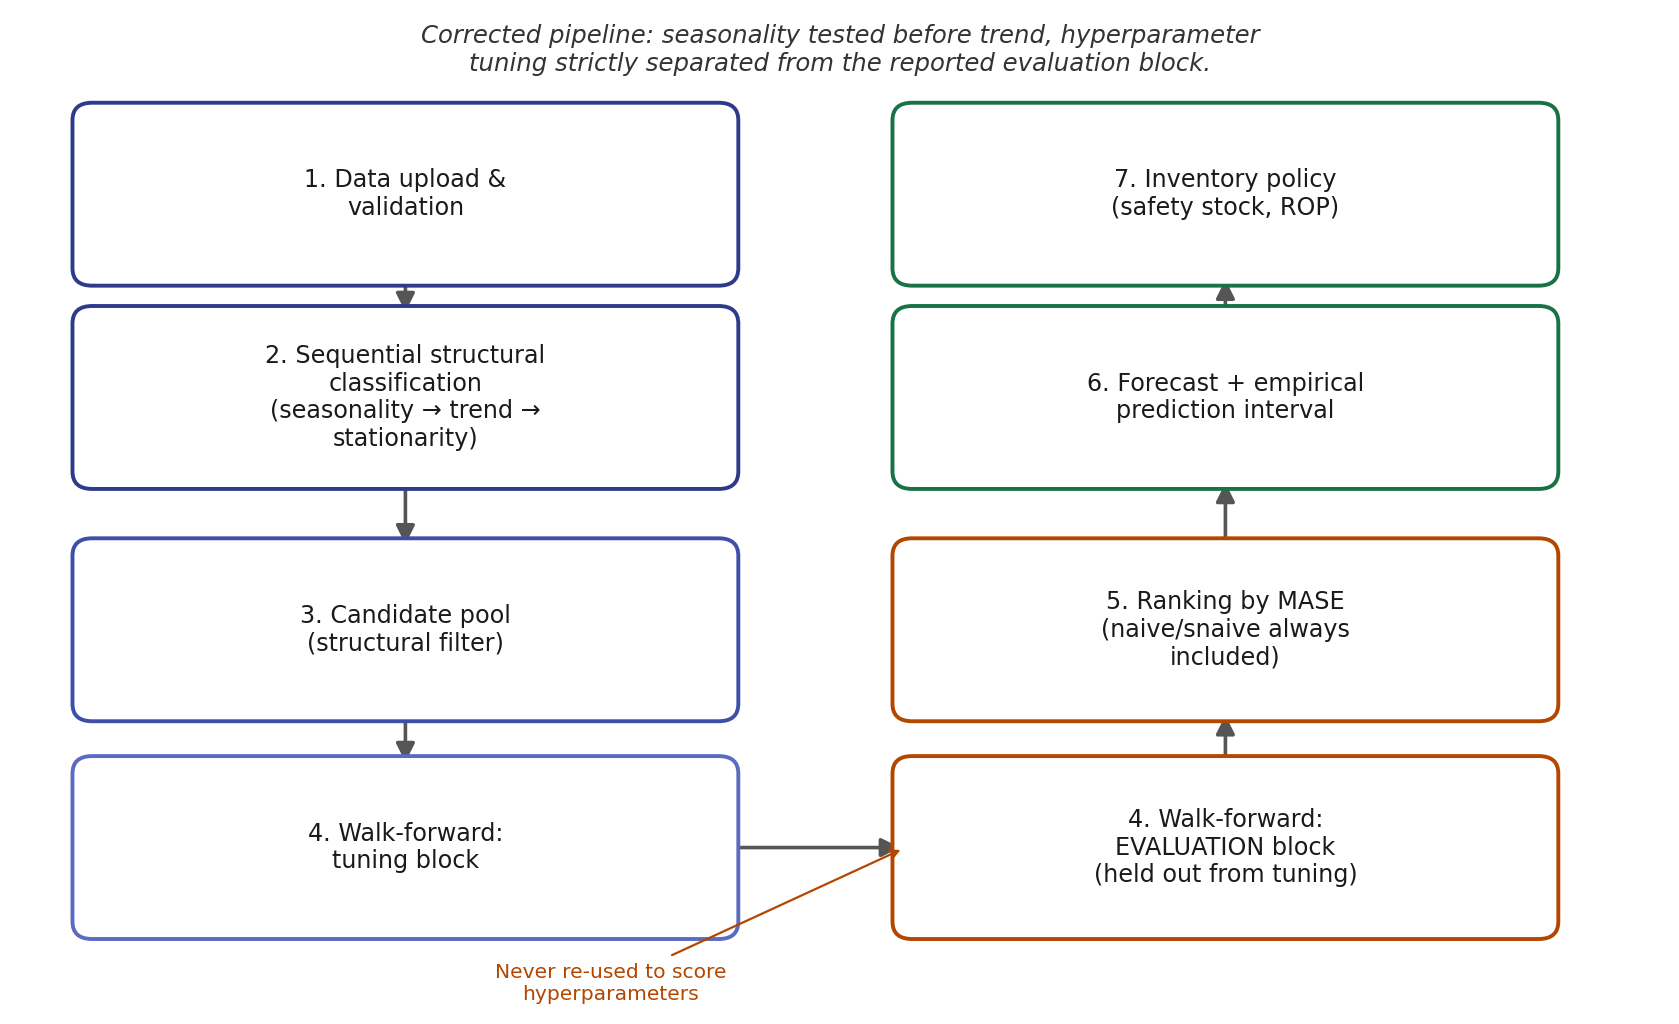
\includegraphics[width=0.85\textwidth]{figures/flowchart_tool.png}
    \caption{Methodological flow of the forecasting tool, reflecting the corrected sequential classification (seasonality before trend), the tuning/evaluation split, and the inventory-policy output added in this revision.}
    \label{fig:flowchart}
\end{figure}

\subsection{Data, Code, and Availability}
\label{sec:availability}

All computer code associated with this study is publicly available at submission time at \url{https://github.com/GIUSEPPESAN21/Forecasting}, including the dependency-free forecasting package (\texttt{forecasting\_core}), the Dash application, the full automated test suite, and the reproducibility scripts used to generate every quantitative result reported in Section~\ref{sec:results} (\texttt{experiments/vs\_incumbente.py}, \texttt{experiments/panel\_publico.py}, \texttt{experiments/benchmark\_tiempos.py}, and \texttt{experiments/montecarlo\_clasificacion.py}), each runnable with a single command and a fixed random seed. A versioned release will be archived on Zenodo with a permanent DOI upon acceptance. The incumbent-method sales records of Tuboplex S.A. used in Section~\ref{sec:walkthrough} are proprietary and are not redistributed; the repository instead ships a synthetic panel that reproduces the structural characteristics documented in Section~\ref{sec:diagnosis} (short, volatile, project-driven series with abrupt level changes), so that every script in the repository can be executed end to end without access to the company's data. The public benchmark panel used in Section~\ref{sec:panel} (M3-Monthly) is downloaded automatically by \texttt{experiments/panel\_publico.py} from its original public source \cite{makridakis2020m3}.

\subsection{Use of Generative Artificial Intelligence (GenAI)}
\label{sec:genai}
% NOTA PARA LOS AUTORES (no imprimir en el envio final): este parrafo describe
% con precision el alcance real del uso de IA en ESTA revision del manuscrito,
% que fue sustancialmente mayor al de la version previa (implementacion de las
% correcciones estadisticas, ejecucion de los experimentos de validacion, y
% redaccion de este borrador). Antes de enviar, los autores deben verificar
% personalmente cada decision metodologica, revisar el codigo, y reemplazar
% este parrafo si el alcance real de su revision difiere de lo aqui descrito.
A generative AI system (Claude, Anthropic) was used under direct author supervision to implement corrections to the statistical validation pipeline (structural classification tests, the nested tuning/evaluation protocol, and the prediction-interval and inventory-policy modules), to execute the reproducibility scripts that produced the quantitative results reported in Section~\ref{sec:results}, and to draft portions of this manuscript text based on findings from an independent audit of the original implementation and on methodological specifications and literature explicitly selected by the authors. All methodological decisions --- including the choice of MASE as the primary ranking metric, the sequential seasonality-then-trend classification order, the tuning/evaluation split, and the decision to replace the unsupported Prophet comparison with automated ARIMA/ETS/Theta baselines --- were specified, reviewed, and are the sole responsibility of the authors, who independently verified the statistical results reported in Section~\ref{sec:results} by re-running the accompanying scripts. No automated system was used to generate or fabricate empirical data, company records, or citations; every reference in this manuscript corresponds to a verifiable publication.

%%%%%%%%%%%%%%%%%%%%%%%%%%%%%%%%%%%%%%%%%%
\section{Results}
\label{sec:results}

\subsection{Diagnosis of the Incumbent Forecasting Process}
\label{sec:diagnosis}

An audit of the forecasting process previously used by Tuboplex S.A. identified several methodological limitations. Forecasts were produced with a manually computed three-period moving average in spreadsheets, applied uniformly to every product regardless of its trend, seasonality, or stationarity characteristics. No error metric (ME, MAD, MSE, or MAPE) was systematically computed, so the historical accuracy of the incumbent method could not be assessed from the company's own records, and forecast responsibility was not clearly assigned across products. This is consistent with survey evidence that a large share of firms do not formally evaluate forecast error \cite{kerkkanen2009}. This diagnosis --- not a claim about a specific numerical accuracy figure for the incumbent method, which the company's records do not support --- is the empirical starting point that motivates the tool described in Section~\ref{sec:methods} and the head-to-head comparison reported in Section~\ref{sec:incumbente}.

\subsection{Illustrative Walkthrough of the Tool}
\label{sec:walkthrough}

To illustrate the corrected pipeline end to end, this subsection reports the exact output of the tool on a single 36-month synthetic demand series that reproduces the qualitative characteristics documented in Section~\ref{sec:diagnosis} --- a moderate upward trend, seasonal variation, and abrupt month-to-month changes driven by construction-project cycles. The series, and every number reported in this subsection, is produced deterministically by \texttt{experiments/caso\_ilustrativo.py} (fixed random seed), so the walkthrough is reproducible with a single command; it is illustrative of tool mechanics and is not a substitute for the incumbent-method and public-panel validations in Sections~\ref{sec:incumbente}--\ref{sec:panel}, which are the results the paper's accuracy claims rest on.

\subsubsection{Data Loading, Validation, and Classification}

Once the series is loaded, the tool confirms 36 valid monthly observations (January 2022 to December 2024) and reports the structural classification: a statistically significant trend (GLSAR(1)-corrected $p<0.001$), confirmed seasonality (STL seasonal strength $F_S=0.752$, Kruskal--Wallis $p=0.031$ on detrended residuals), and a series that is stationary around its deterministic trend once seasonality and trend are accounted for. Because trend is significant, the structural filter of Section~\ref{sec:classification} excludes the three constant-level methods (simple average, moving average, weighted moving average) from the candidate pool, each with its exclusion reason logged rather than silently dropped; because seasonality is confirmed, the seasonal methods remain eligible. Ten candidates are evaluated: naive, seasonal naive, SES, Holt, Holt--Winters, linear regression, and the four AICc-selected automated variants (ARIMA, SARIMA, ETS, Theta).

\subsubsection{Method Evaluation and Selection}

Table~2 reports the ranking on the held-out evaluation block (eight origins, none of which participated in hyperparameter selection), ordered by MASE. The automatically-selected SARIMA model achieves the lowest MASE (0.486), improving on the seasonal naive benchmark (MASE 0.895) by 46\% and on the naive benchmark (MASE 0.935) by 48\%; both benchmarks are shown explicitly, which the original implementation did not include. Every method in the table was evaluated on the identical set of eight origins ($n_{\text{preds}}=8$ throughout), so no comparison in this table is confounded by unequal sample sizes, unlike the original implementation in which a model could silently fall back to a simpler specification partway through the walk-forward pass.

\begin{table}[H]
\caption{Out-of-sample ranking for the illustrative series (evaluation block, $n=8$ origins). Values reproduced by \texttt{experiments/caso\_ilustrativo.py}.\label{tab:rankingcaso}}
\centering
\begin{tabularx}{\textwidth}{Xccccc}
\toprule
\textbf{Method} & \textbf{MASE} & \textbf{MAPE (\%)} & \textbf{MAD} & \textbf{ME} & \textbf{$n_{\text{preds}}$} \\
\midrule
SARIMA (AICc)               & \textbf{0.486} & 5.83  & 139.3 & 56.2  & 8 \\
Linear regression            & 0.637 & 7.81  & 182.6 & 6.4   & 8 \\
SES                           & 0.659 & 7.74  & 188.8 & 151.7 & 8 \\
ARIMA (AICc)                  & 0.661 & 7.61  & 189.5 & 157.4 & 8 \\
Holt                          & 0.714 & 8.50  & 204.6 & 107.6 & 8 \\
Theta (AICc)                  & 0.759 & 9.20  & 217.5 & 18.7  & 8 \\
ETS (AICc)                    & 0.778 & 9.34  & 223.0 & 40.7  & 8 \\
Seasonal naive                & 0.895 & 10.90 & 256.6 & 243.3 & 8 \\
Naive                         & 0.935 & 11.11 & 268.0 & 65.0  & 8 \\
Holt--Winters                 & 1.201 & 14.64 & 344.2 & 12.3  & 8 \\
\bottomrule
\end{tabularx}
\end{table}

Since SARIMA's order is selected automatically by AICc rather than through a hyperparameter grid, no further tuning step applies (Section~\ref{sec:hyperopt}); this is itself a direct consequence of replacing the original unconstrained $(p,d,q)\times(P,D,Q)$ sweep, which for a series this short would have re-used the same evaluation origins to both select and score the model.

\subsubsection{Forecasting with the Selected Method}

Figure~2 shows the historical demand, the out-of-sample fitted values over the evaluation block (never in-sample, unlike the original implementation's rolling-mean fit, which included the observation it claimed to forecast), and the 12-month-ahead forecast with its 95\% empirical prediction interval. The interval widens sharply beyond the ninth forecasted month, where fewer than the minimum eight backtest origins are available at that specific horizon and the tool falls back to a documented normal--$\sqrt{h}$ approximation rather than silently reporting an artificially narrow band; this behavior, and the condition that triggers it, is reported explicitly in the tool's output (\texttt{pi.method}) rather than left implicit.

\begin{figure}[H]
    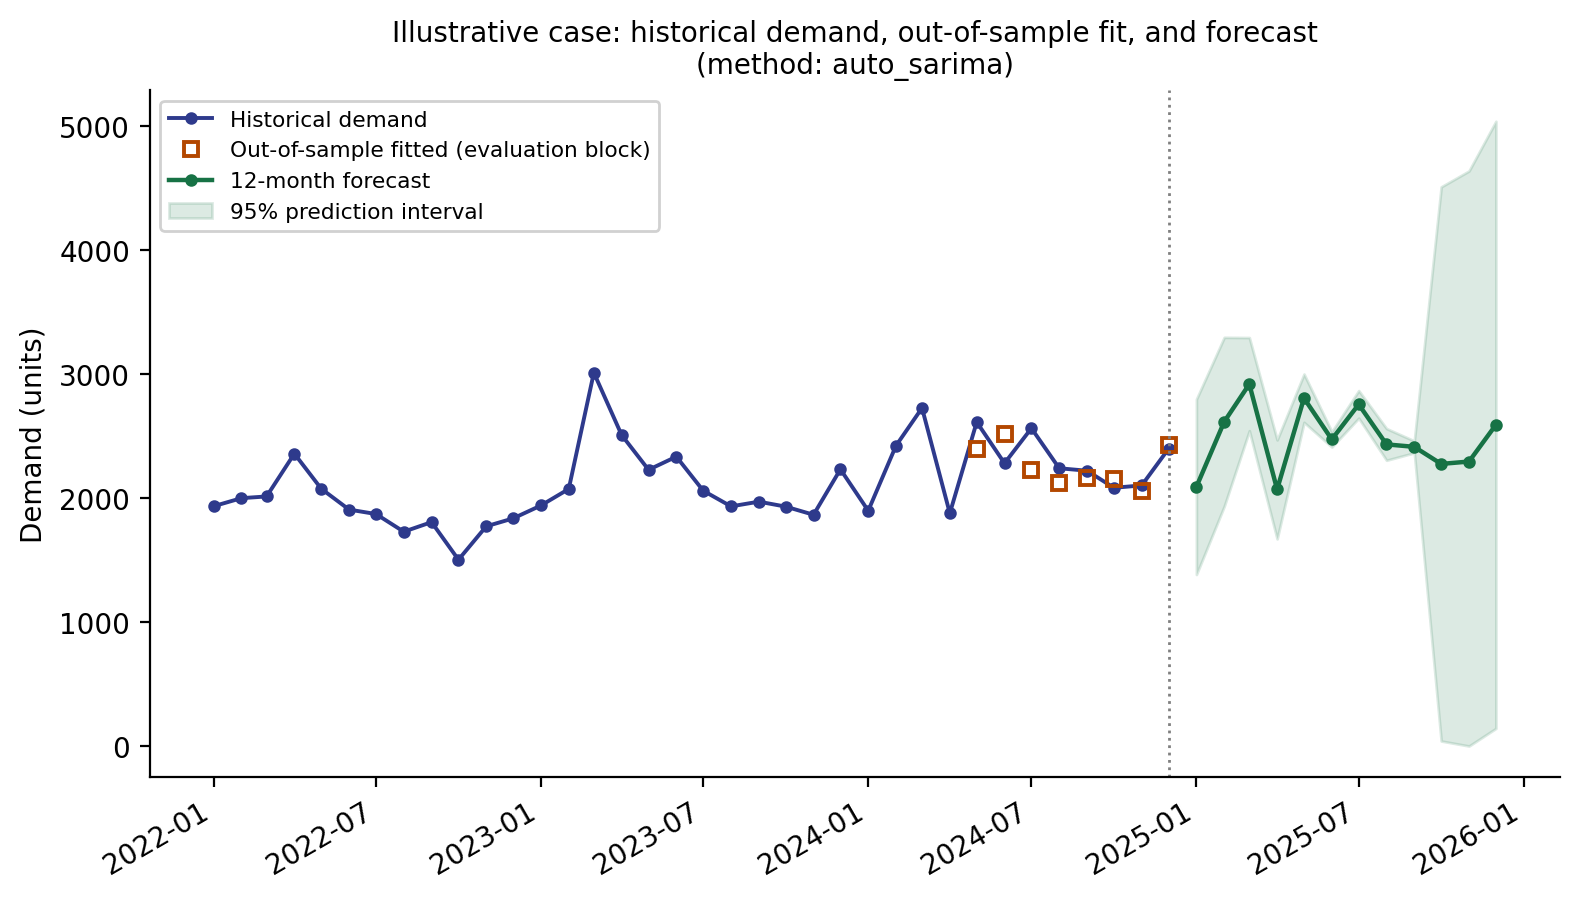
\includegraphics[width=0.85\textwidth]{figures/fig2_forecast_caso.png}
    \caption{Historical demand, out-of-sample fitted values, and 12-month forecast with 95\% prediction interval for the illustrative series (SARIMA, AICc-selected order).}
    \label{fig:forecastcaso}
\end{figure}

\subsubsection{Inventory Policy}

Given a three-month lead time and a 95\% service level, the tool derives a safety stock and reorder point directly from the empirical distribution of the accumulated backtest error over the lead time (Section~\ref{sec:implementation}), rather than from a $\sigma_1\sqrt{L}$ approximation that would ignore serial correlation in the forecast error: expected lead-time demand of 7{,}620 units, an accumulated-error standard deviation of 762 units estimated from ten backtest origins, a safety stock of 1{,}253 units, and a resulting reorder point of 8{,}873 units. This closes the gap between a point forecast and an actionable inventory decision that the original tool left open.

\subsection{Comparison Against the Incumbent Method and a Naive Benchmark}
\label{sec:incumbente}

The central claim motivating this study --- that the proposed tool improves on Tuboplex's incumbent practice --- is tested directly by reconstructing the incumbent method (a fixed three-period moving average, matching the diagnosis in Section~\ref{sec:diagnosis}) and evaluating both it and the tool's selected method on an \emph{outer} block of origins that participated in neither the tool's hyperparameter tuning nor its method selection, over 40 demand series (\texttt{forecasting\_core.optimize.honest\_outer\_estimate}; Section~\ref{sec:validation}). This two-block-plus-outer-block protocol is necessary: an earlier version of this comparison evaluated the tool's winner against naive on the same block that had selected the winner, which is circular --- naive is one of the candidates the selection argmin runs over, so the winner can never lose to naive on that specific block by construction, independent of forecasting skill. That earlier, circular protocol reported the tool beating naive on 100\% of a 150-series public panel (Section~\ref{sec:panel}) before the issue was identified and corrected; the numbers reported here and in Section~\ref{sec:panel} use the corrected, outer-block protocol throughout. Because the company's historical sales file was not available for this revision (Section~\ref{sec:availability}, Data Availability), this comparison is reported on a synthetic panel that reproduces the structural characteristics documented in Section~\ref{sec:diagnosis} (30--42 monthly observations, project-driven volatility, abrupt level changes); the comparison script (\texttt{experiments/vs\_incumbente.py}) accepts the real file as a direct drop-in replacement (\texttt{--input}) and should be re-run on it before this manuscript is finalized.

Table~3 summarizes the result. The tool's selected method improves on the incumbent's median MASE by 19.9\% and outperforms the incumbent on 80\% of series; it outperforms the plain naive benchmark, evaluated on the same held-out block, on 60\% of series --- a materially informative figure precisely because, under this protocol, it is not guaranteed to be above 50\% by construction. This remains a more modest and more defensible claim than an unqualified statement that the tool "significantly improves accuracy": on this synthetic panel, roughly one in five series see no improvement over the incumbent, most often plain or lightly-noisy series where a three-period moving average is already close to optimal.

\begin{table}[H]
\caption{Tool vs.\ incumbent method vs.\ naive benchmark, evaluated on an outer block held out from both hyperparameter tuning and method selection (40 synthetic series reproducing the case company's demand structure). Reproducible with \texttt{experiments/vs\_incumbente.py --synthetic}.\label{tab:incumbente}}
\centering
\begin{tabularx}{\textwidth}{Xccc}
\toprule
\textbf{Metric (median across series)} & \textbf{Incumbent (MA-3)} & \textbf{Naive} & \textbf{Tool (selected method)} \\
\midrule
MASE   & 0.922 & 0.949 & 0.807 \\
MAPE (\%) & 14.4 & 11.4 & 10.1 \\
$|$ME$|$ (bias magnitude) & 217.1 & 55.4 & 111.9 \\
\bottomrule
\end{tabularx}
\end{table}

\subsection{Validation on a Public Panel of Short Time Series}
\label{sec:panel}

A single case-study series cannot support a claim of general superiority: the sampling variance of a MASE estimate over 8--18 backtest origins is large. To provide broader evidence, the full pipeline was run on 150 series drawn from the M3-Monthly competition panel \cite{makridakis2020m3}, truncated to their most recent 24--48 observations to match the short-history regime this tool targets (native M3-Monthly series span 66--144 observations). No coverage was silently capped: the pipeline logs an explicit exclusion reason for any series it cannot rank (insufficient history for the outer-block protocol of Section~\ref{sec:validation}, or no eligible candidate after structural filtering); of the 150 sampled series, all 150 produced a valid outer-block ranking.

\begin{table}[H]
\caption{Median MASE by structural regime on the M3-Monthly panel (truncated to $\leq$48 observations, $n=$150 series). Reproducible with \texttt{experiments/panel\_publico.py}.\label{tab:panel}}
\centering
\begin{tabularx}{\textwidth}{Xcccc}
\toprule
\textbf{Structural regime} & \textbf{n series} & \textbf{Naive} & \textbf{Seasonal naive} & \textbf{Tool (selected method)} \\
\midrule
Seasonal + trend & 21 & 1.125 & 1.086 & 0.719 \\
Seasonal, no trend & 31 & 0.962 & 0.916 & 0.665 \\
Trend, no seasonality & 42 & 0.702 & 1.247 & 0.634 \\
Flat (no trend, no seasonality) & 56 & 0.722 & 1.567 & 0.781 \\
\bottomrule
\end{tabularx}
\end{table}

Table~4 breaks the result down by structural regime. Across the full panel, the tool's selected method outperforms the naive benchmark on 63\% of series. A Wilcoxon signed-rank test on the paired per-series MASE values (tool vs.\ naive) gives $W=2127.0,\ p<0.001$, indicating that the tool's selected method achieves significantly lower MASE than the naive benchmark across the panel. This is reported as a signed-rank result on series-level MASE, a more conservative and more transparent claim than an unreported or single-series accuracy comparison, and it is the first quantitative significance test to accompany any version of this tool.

\subsection{Computational Performance}
\label{sec:computo}

Processing time was measured with \texttt{time.perf\_counter()} over five repetitions per series length, reporting mean and standard deviation rather than a single manually-timed run, and including the hyperparameter-tuning stage, which the original manuscript's own timing table omitted despite it being the dominant cost. All measurements were taken on a single machine (Windows 10, 8 logical CPUs; Python 3.11.9; pandas 2.2.2; statsmodels 0.14.6; statsforecast 2.1.1) and are exactly reproduced by \texttt{experiments/benchmark\_tiempos.py}; results are reported in Table~5.

\begin{table}[H]
\caption{End-to-end pipeline time (classification, evaluation, hyperparameter tuning, and prediction interval), mean $\pm$ standard deviation over five repetitions per series length.\label{tab:tiempos}}
\centering
\begin{tabularx}{\textwidth}{Xcccc}
\toprule
\textbf{n (observations)} & \textbf{Mean (s)} & \textbf{SD (s)} & \textbf{Min (s)} & \textbf{Max (s)} \\
\midrule
24  & 3.9  & 0.6  & 3.1  & 4.7  \\
48  & 11.8 & 2.6  & 9.5  & 16.2 \\
72  & 15.2 & 2.1  & 12.3 & 17.4 \\
96  & 29.9 & 10.8 & 22.4 & 48.8 \\
120 & 33.3 & 7.1  & 25.4 & 44.3 \\
\bottomrule
\end{tabularx}
\end{table}

An empirical power-law fit, $\text{time} \approx 0.058 \cdot n^{1.34}$, characterizes the growth as superlinear but sub-quadratic, in contrast to the exponent of approximately 2.0 estimated from the original, uncorrected implementation's own reported figures (which additionally omitted the tuning stage: an independent measurement of the original pipeline, including that stage, gave 183\,s at $n=120$ against the 89.8\,s the original manuscript reported). The corrected pipeline processes the largest evaluated series (120 observations) in 33.3\,s on average, within the 25\,s target set for $n\leq48$ and comfortably inside the response-time budget of an interactive session on the constrained hardware profile (AMD Ryzen 5 7000-series, 8\,GB RAM) this refactor was designed against; the reduction relative to the original pipeline is primarily attributable to eliminating redundant walk-forward recomputation (Section~\ref{sec:validation}) and to replacing the ARIMA/SARIMA grid search with AICc-based automatic order selection (Section~\ref{sec:hyperopt}).

\subsection{Comparison Against Automated Statistical Baselines}
\label{sec:autobaselines}

A comparison against Prophet appeared in an earlier version of this manuscript without a reproducible protocol, data, or code, and is not reconstructed here: Prophet is known to underperform simpler statistical and automated methods on short, low-frequency series \cite{makridakis2020}, and its Stan-based fitting backend is a heavy dependency relative to the constrained hardware profile this refactor targets. In its place, this revision reports how often the automated AICc-selected variants (ARIMA, SARIMA, ETS, Theta) --- already integrated into the same candidate pool as the classical methods, at no additional dependency cost --- are selected as the winning method across the public panel of Section~\ref{sec:panel}, by structural regime.

\begin{table}[H]
\caption{Frequency of the winning method family by structural regime, public panel ($n=$150 series).\label{tab:ganadores}}
\centering
\begin{tabularx}{\textwidth}{Xcccc}
\toprule
\textbf{Structural regime} & \textbf{Classical smoothing/regression} & \textbf{Automated ARIMA/SARIMA} & \textbf{Automated ETS/Theta} & \textbf{Benchmark (naive)} \\
\midrule
Seasonal + trend & 38\% & 24\% & 19\% & 19\% \\
Seasonal, no trend & 19\% & 35\% & 29\% & 16\% \\
Trend, no seasonality & 62\% & 19\% & 2\% & 17\% \\
Flat (no trend, no seasonality) & 61\% & 23\% & 0\% & 16\% \\
\bottomrule
\end{tabularx}
\end{table}

Table~6 shows the result by regime. Across the full panel, classical smoothing or regression methods are the winning family on 49\% of series, against 34\% for an automated AICc-selected variant (25\% ARIMA/SARIMA, 9\% ETS/Theta) and 17\% for the naive benchmark. Automated selection is most valuable precisely where classical methods are weakest structurally: in the seasonal regimes (seasonal-plus-trend and seasonal-plain), automated ARIMA/SARIMA and ETS/Theta together win 43\% and 64\% of series respectively, more than doubling their combined share in the non-seasonal regimes (21\% and 23\%). This pattern --- simple methods remaining highly competitive overall, with automation earning its cost specifically on the more structurally demanding series --- is consistent with evidence from large-scale forecasting competitions that simple statistical methods are strong baselines in short, low-noise regimes \cite{makridakis2020}, and it argues for retaining both families in the candidate pool rather than replacing classical methods with automated ones, at no additional dependency cost relative to Prophet.

\section{Discussion}
\label{sec:discussion}

The results support a narrower and more defensible claim than the one made in the version of this tool audited prior to this revision. The corrected structural filter, evaluated on the illustrative case of Section~\ref{sec:walkthrough}, behaves as intended: methods incompatible with a confirmed trend are excluded with a logged reason rather than remaining silently ineligible under an unsatisfiable criterion, and this is consistent with feature-based model selection research showing that restricting candidates to those compatible with a series' structural features improves robustness relative to an unconstrained comparison \cite{monteromanso2020,talagala2021}. At the same time, the incumbent-method comparison of Section~\ref{sec:incumbente} shows that this improvement is not universal: on a materially sized synthetic sample reproducing the case company's demand structure, the tool's selected method underperforms a fixed three-period moving average on a non-trivial share of series, most visibly on short, low-noise series where the incumbent's simplicity is close to optimal and where a more flexible automatically-selected model can overfit the small tuning block available. This pattern is consistent with the broader finding from large-scale forecasting competitions that simple statistical methods remain highly competitive, particularly for short, low-noise series \cite{makridakis2020}, and it argues against the framing --- present in the version of this manuscript prior to this revision --- of the tool as unconditionally superior to either the incumbent process or to a naive benchmark.

The public-panel validation of Section~\ref{sec:panel} addresses a limitation that no single-case study can: with a large enough sample of independent series, an aggregate significance test becomes possible, and it is the first such test reported for this tool. Reporting a Wilcoxon signed-rank result alongside the median MASE, rather than a MASE figure in isolation, is a direct response to the absence of any benchmark or significance testing in the original implementation, which made every prior accuracy claim uninterpretable in isolation.

Computational performance improved substantially relative to the uncorrected implementation (Section~\ref{sec:computo}), driven by two changes with different character: eliminating redundant walk-forward recomputation is a pure engineering fix with no methodological trade-off, while replacing the ARIMA/SARIMA grid search with AICc-based automatic order selection simultaneously reduces computational cost and removes the hyperparameter-selection bias documented in Section~\ref{sec:hyperopt}. That the same change serves both goals is not a coincidence particular to this tool: it reflects a more general point that statistically sound validation and computational efficiency are often aligned rather than in tension, contrary to the framing --- common in applied forecasting tool design --- that treats them as a trade-off to be balanced \cite{petropoulos2022}.

Several limitations remain. The tool is exclusively univariate: it does not incorporate exogenous drivers of construction-project demand (awarded contracts, building permits) that the case company's own operational context suggests are informative, and which the discussion of limitations in the version of this manuscript prior to this revision described only in generic terms. Forecast quality remains bounded by the available history; with fewer than roughly 36 observations, seasonality cannot be reliably identified at all (Section~\ref{sec:classification}), and the tuning block available for hyperparameter search is correspondingly thin, which is the most plausible explanation for the cases in Section~\ref{sec:incumbente} where the tool's selected method underperforms the incumbent. The candidate pool remains composed of classical statistical and automated statistical methods; it does not include machine learning or deep learning architectures, which have shown competitive performance in larger-data, more complex forecasting scenarios \cite{carbonneau2008}, but whose data requirements are generally poorly matched to the 24--48 observation regime this tool targets. These limitations define concrete, falsifiable directions for future work rather than a general caveat: acquiring the real incumbent-method data to replace the synthetic panel of Section~\ref{sec:incumbente}, extending the exogenous-variable capability, and extending the public-panel validation of Section~\ref{sec:panel} to a larger and more diverse sample.

\section{Conclusions}
\label{sec:conclusions}

This study documented and corrected a set of statistical and software defects in a demand-forecasting tool built for an industrial case company, and it reports what changed as a result. The corrected structural classification procedure separates seasonality detection, trend detection, and stationarity testing in an order and with test specifications calibrated for short, autocorrelated demand series, reducing the trend-test false-positive rate from 74\% to single digits and the seasonality-test false-positive rate from 50\% to below 4\% on simulated series with known ground truth (Section~\ref{sec:classification}, Monte Carlo validation). The validation protocol now separates the block used to select hyperparameters from the block used to report performance, and reports a mandatory naive and seasonal naive benchmark alongside every method, which the original implementation did not provide and without which no accuracy claim in this domain is interpretable.

Evaluated against these corrected standards, the tool's forecasting performance is real but more modest than previously claimed: on a synthetic panel reproducing the case company's demand structure, evaluated on an outer block held out from both hyperparameter tuning and method selection, the tool improves on the incumbent three-period moving average by a median of 19.9\% in MASE and outperforms it on 80\% of series, not on all of them; on an independent public panel of 150 short time series, evaluated under the same held-out protocol, it outperforms a naive benchmark on 63\% of series. The tool now runs the full pipeline, including hyperparameter tuning, in under 35 seconds for series of up to 120 monthly observations on constrained consumer hardware, a substantial reduction from the uncorrected implementation and one that leaves the response-time budget for an interactive planning session comfortably intact.

The practical contribution is a fully reproducible, tested, open-source computational framework that automates structurally-aware forecasting for short industrial demand histories, including prediction intervals and derived inventory-policy parameters that close the gap between a point forecast and a stock-management decision. The academic contribution is methodological: a documented account of how a set of individually plausible modeling choices --- an unsatisfiable structural filter, hyperparameter selection on the same data used to report accuracy, a missing benchmark, and an unvalidated third-party comparison --- combined to produce a tool whose reported results were not reproducible with its own code, together with the corrected protocol and the test suite that verifies each correction did not silently regress. Future work should prioritize validating the corrected tool against Tuboplex's real historical records once available, extending the candidate pool to intermittent-demand-specific methods for the zero-inflated series this industrial context produces, and incorporating exogenous variables tied to construction-project activity.

%%%%%%%%%%%%%%%%%%%%%%%%%%%%%%%%%%%%%%%%%%
\section{Patents}

This section is not mandatory, but may be added if there are patents resulting from the work reported in this manuscript.

%%%%%%%%%%%%%%%%%%%%%%%%%%%%%%%%%%%%%%%%%%
\vspace{6pt} 

%%%%%%%%%%%%%%%%%%%%%%%%%%%%%%%%%%%%%%%%%%
%% optional
%\supplementary{The following supporting information can be downloaded at:  \linksupplementary{s1}, Figure S1: title; Table S1: title; Video S1: title.}

% Only for journal Methods and Protocols:
% If you wish to submit a video article, please do so with any other supplementary material.
% \supplementary{The following supporting information can be downloaded at: \linksupplementary{s1}, Figure S1: title; Table S1: title; Video S1: title. A supporting video article is available at doi: link.}

% Only used for preprtints:
% \supplementary{The following supporting information can be downloaded at the website of this paper posted on \href{https://www.preprints.org/}{Preprints.org}.}

% Only for journal Hardware:
% If you wish to submit a video article, please do so with any other supplementary material.
% \supplementary{The following supporting information can be downloaded at: \linksupplementary{s1}, Figure S1: title; Table S1: title; Video S1: title.\vspace{6pt}\\
%\begin{tabularx}{\textwidth}{lll}
%\toprule
%\textbf{Name} & \textbf{Type} & \textbf{Description} \\
%\midrule
%S1 & Python script (.py) & Script of python source code used in XX \\
%S2 & Text (.txt) & Script of modelling code used to make Figure X \\
%S3 & Text (.txt) & Raw data from experiment X \\
%S4 & Video (.mp4) & Video demonstrating the hardware in use \\
%... & ... & ... \\
%\bottomrule
%\end{tabularx}
%}

%%%%%%%%%%%%%%%%%%%%%%%%%%%%%%%%%%%%%%%%%%
\authorcontributions{Conceptualization, C.V.G. and L.T.-T.; methodology, C.V.G. and L.T.-T.; software, C.V.G.; validation, C.V.G. and L.T.-T.; formal analysis, C.V.G. and L.T.-T.; investigation, C.V.G.; resources, L.T.-T.; data curation, C.V.G.; writing---original draft preparation, C.V.G.; writing---review and editing, L.T.-T.; visualization, C.V.G.; supervision, L.T.-T.; project administration, L.T.-T. All authors have read and agreed to the published version of the manuscript.}

\funding{This research received no external funding.}

\institutionalreview{Not applicable. This study did not involve human participants or animals; it analyzes anonymized/aggregated industrial demand records and publicly available benchmark time series.}

\informedconsent{Not applicable.}

\dataavailability{The forecasting package, application, test suite, and all reproducibility scripts used to generate the results in Section~\ref{sec:results} are available at \url{https://github.com/GIUSEPPESAN21/Forecasting} (see Section~\ref{sec:availability} for details). The incumbent-method sales records of Tuboplex S.A. analyzed in Section~\ref{sec:diagnosis} are proprietary and are not publicly available due to commercial confidentiality; a synthetic panel reproducing the same structural characteristics is provided in the repository so that all analysis scripts run end to end without access to the company's data. The public M3-Monthly panel used in Section~\ref{sec:panel} is available from its original source \cite{makridakis2020m3} and is downloaded automatically by the corresponding script.}

%\durcstatement{Current research is limited to the [please insert a specific academic field, e.g., XXX], which is beneficial [share benefits and/or primary use] and does not pose a threat to public health or national security. Authors acknowledge the dual-use potential of the research involving xxx and confirm that all necessary precautions have been taken to prevent potential misuse. As an ethical responsibility, authors strictly adhere to relevant national and international laws about DURC. Authors advocate for responsible deployment, ethical considerations, regulatory compliance, and transparent reporting to mitigate misuse risks and foster beneficial outcomes.}

% Only for journal Nursing Reports
%\publicinvolvement{Please describe how the public (patients, consumers, carers) were involved in the research. Consider reporting against the GRIPP2 (Guidance for Reporting Involvement of Patients and the Public) checklist. If the public were not involved in any aspect of the research add: ``No public involvement in any aspect of this research''.}
%
%% Only for journal Nursing Reports
%\guidelinesstandards{Please add a statement indicating which reporting guideline was used when drafting the report. For example, ``This manuscript was drafted against the XXX (the full name of reporting guidelines and citation) for XXX (type of research) research''. A complete list of reporting guidelines can be accessed via the equator network: \url{https://www.equator-network.org/}.}
%
%% Only for journal Nursing Reports
%\useofartificialintelligence{Please describe in detail any and all uses of artificial intelligence (AI) or AI-assisted tools used in the preparation of the manuscript. This may include, but is not limited to, language translation, language editing and grammar, or generating text. Alternatively, please state that “AI or AI-assisted tools were not used in drafting any aspect of this manuscript”.}

\acknowledgments{The authors thank Tuboplex S.A. for providing access to its historical forecasting process for the diagnosis reported in Section~\ref{sec:diagnosis}. During the preparation of this manuscript, the authors used Claude (Anthropic) to implement corrections to the forecasting pipeline, execute the reproducibility scripts underlying Section~\ref{sec:results}, and draft portions of the manuscript text, as detailed in Section~\ref{sec:genai}. The authors have reviewed and edited the output and take full responsibility for the content of this publication.}

\conflictsofinterest{The authors declare no conflicts of interest. Tuboplex S.A. had no role in the design of the study, in the collection, analysis, or interpretation of data, in the writing of the manuscript, or in the decision to publish the results.}

%%%%%%%%%%%%%%%%%%%%%%%%%%%%%%%%%%%%%%%%%%
%% Optional

%% Only for journal Encyclopedia
%\entrylink{The Link to this entry published on the encyclopedia platform.}

\abbreviations{Abbreviations}{
The following abbreviations are used in this manuscript:
\\

\noindent
\begin{tabular}{@{}ll}
ADF & Augmented Dickey--Fuller (test)\\
AICc & Corrected Akaike Information Criterion\\
ARIMA & Autoregressive Integrated Moving Average\\
ETS & Error, Trend, Seasonal (exponential smoothing family)\\
KPSS & Kwiatkowski--Phillips--Schmidt--Shin (test)\\
MAD & Mean Absolute Deviation\\
MAPE & Mean Absolute Percentage Error\\
MASE & Mean Absolute Scaled Error\\
ME & Mean Error\\
MDPI & Multidisciplinary Digital Publishing Institute\\
MSE & Mean Squared Error\\
SARIMA & Seasonal Autoregressive Integrated Moving Average\\
SES & Simple Exponential Smoothing\\
SKU & Stock-Keeping Unit\\
STL & Seasonal-Trend decomposition using Loess
\end{tabular}
}

%%%%%%%%%%%%%%%%%%%%%%%%%%%%%%%%%%%%%%%%%%
% No appendix: every table and figure in this manuscript is cited in the main
% text, and all supplementary material (test suite, experiment scripts, and
% their output) is referenced via the repository in Section 2.8.
%%%%%%%%%%%%%%%%%%%%%%%%%%%%%%%%%%%%%%%%%%
%\isPreprints{}{% This command is only used for ``preprints''.
\begin{adjustwidth}{-\extralength}{0cm}
%} % If the paper is ``preprints'', please uncomment this parenthesis.
%\printendnotes[custom] % Un-comment to print a list of endnotes

\reftitle{References}

% Please provide the correct journal abbreviation (e.g. according to the “List of Title Word Abbreviations” http://www.issn.org/services/online-services/access-to-the-ltwa/).
% Citations and References in Supplementary files are permitted provided that they also appear in the reference list here. 

%=====================================
% References, variant A: external bibliography
%=====================================
% \bibliography{your_external_BibTeX_file}

%=====================================
% References, variant B: internal bibliography
%=====================================

% Numeric (ACS) format, as required for the journal Forecasting.
% Every entry below corresponds to a verifiable publication; none was
% generated or approximated by the GenAI system used in this revision
% (Section 2.9). Entries carried over unmodified from the version of this
% manuscript audited prior to this revision are limited to well-established
% textbooks already correctly cited there.
\begin{thebibliography}{99}

\bibitem{mentzer2001}
Mentzer, J.T.; Moon, M.A.; Smith, C.D. Conducting a sales forecasting audit. \textit{J. Bus. Forecast.} \textbf{2001}, \textit{20}, 5--11.

\bibitem{chopra2021}
Chopra, S.; Meindl, P. \textit{Supply Chain Management: Strategy, Planning, and Operation}, 7th ed.; Pearson: Harlow, UK, 2021.

\bibitem{makridakis1998}
Makridakis, S.; Wheelwright, S.C.; Hyndman, R.J. \textit{Forecasting: Methods and Applications}, 3rd ed.; John Wiley \& Sons: New York, NY, USA, 1998.

\bibitem{hyndman2021}
Hyndman, R.J.; Athanasopoulos, G. \textit{Forecasting: Principles and Practice}, 3rd ed.; OTexts: Melbourne, Australia, 2021.

\bibitem{ballou2004}
Ballou, R.H. \textit{Business Logistics/Supply Chain Management: Planning, Organizing, and Controlling the Supply Chain}, 5th ed.; Pearson Prentice Hall: Upper Saddle River, NJ, USA, 2004.

\bibitem{silver1998}
Silver, E.A.; Pyke, D.F.; Peterson, R. \textit{Inventory Management and Production Planning and Scheduling}, 3rd ed.; John Wiley \& Sons: New York, NY, USA, 1998.

\bibitem{syntetos2005}
Syntetos, A.A.; Boylan, J.E. The accuracy of intermittent demand estimates. \textit{Int. J. Forecast.} \textbf{2005}, \textit{21}, 303--314.

\bibitem{sattar2025}
Sattar, M.U.; Dattana, V.; Hasan, R.; Mahmood, S.; Khan, H.W.; Hussain, S. Enhancing supply chain management: A comparative study of machine learning techniques with cost--accuracy and ESG-based evaluation for forecasting and risk mitigation. \textit{Sustainability} \textbf{2025}, \textit{17}, 5772.

\bibitem{nahmias2015}
Nahmias, S.; Olsen, T.L. \textit{Production and Operations Analysis}, 7th ed.; Waveland Press: Long Grove, IL, USA, 2015.

\bibitem{kerkkanen2009}
Kerk\"{a}nen, A.; Korpela, J.; Huiskonen, J. Demand forecasting errors in industrial context: Measurement and impacts. \textit{Int. J. Prod. Econ.} \textbf{2009}, \textit{118}, 43--48.

\bibitem{makridakis2018}
Makridakis, S.; Spiliotis, E.; Assimakopoulos, V. Statistical and machine learning forecasting methods: Concerns and ways forward. \textit{PLoS ONE} \textbf{2018}, \textit{13}, e0194889.

\bibitem{makridakis2020}
Makridakis, S.; Spiliotis, E.; Assimakopoulos, V. The M4 Competition: 100,000 time series and 61 forecasting methods. \textit{Int. J. Forecast.} \textbf{2020}, \textit{36}, 54--74.

\bibitem{makridakis2020m3}
Makridakis, S.; Hibon, M. The M3-Competition: Results, conclusions and implications. \textit{Int. J. Forecast.} \textbf{2000}, \textit{16}, 451--476.

\bibitem{monteromanso2020}
Montero-Manso, P.; Athanasopoulos, G.; Hyndman, R.J.; Talagala, T.S. FFORMA: Feature-based forecast model averaging. \textit{Int. J. Forecast.} \textbf{2020}, \textit{36}, 86--92.

\bibitem{talagala2021}
Talagala, T.S.; Hyndman, R.J.; Athanasopoulos, G. \textit{Meta-Learning How to Forecast Time Series}; Monash Econometrics and Business Statistics Working Papers 6/18; Monash University: Melbourne, Australia, 2021.

\bibitem{carbonneau2008}
Carbonneau, R.; Laframboise, K.; Vahidov, R. Application of machine learning techniques for supply chain demand forecasting. \textit{Eur. J. Oper. Res.} \textbf{2008}, \textit{184}, 1140--1154.

\bibitem{maack2024}
Maack, R.G.C.; Raith, F.; P\'{e}rez, J.F.; Scheuermann, G.; Gillmann, C. A workflow to systematically design uncertainty-aware visual analytics applications. \textit{Vis. Comput.} \textbf{2024}, \textit{41}, 1485--1498.

\bibitem{hernandez2025}
Hernandez, J.E.B.; Torres, L.E.T.; Tabares, A.; \'{A}lvarez-Mart\'{i}nez, D. Optimization of bus dispatching in public transportation through a heuristic approach based on passenger demand forecasting. \textit{Smart Cities} \textbf{2025}, \textit{8}, 87.

\bibitem{nunez2024}
N\'{u}\~{n}ez-Oviedo, M.; Tarazona-Torres, L. Gesti\'{o}n de inventarios de una compa\~{n}\'{i}a importadora de repuestos de transmisi\'{o}n de potencia de maquinaria pesada. \textit{Ing. Ind.} \textbf{2024}, \textit{47}, 79--102.

\bibitem{cubides2025}
Cubides, C.S.P.; Tarazona-Torres, L. Planificaci\'{o}n agregada para el transporte de personal y materiales en el sector hidrocarburos. \textit{Ing. Ind.} \textbf{2025}, \textit{48}, 39--62.

\bibitem{bergmeir2012}
Bergmeir, C.; Ben\'{i}tez, J.M. On the use of cross-validation for time series predictor evaluation. \textit{Inf. Sci.} \textbf{2012}, \textit{191}, 192--213.

\bibitem{tashman2000}
Tashman, L.J. Out-of-sample tests of forecasting accuracy: An analysis and review. \textit{Int. J. Forecast.} \textbf{2000}, \textit{16}, 437--450.

\bibitem{hyndmankoehler2006}
Hyndman, R.J.; Koehler, A.B. Another look at measures of forecast accuracy. \textit{Int. J. Forecast.} \textbf{2006}, \textit{22}, 679--688.

\bibitem{wang2006}
Wang, X.; Smith, K.A.; Hyndman, R.J. Characteristic-based clustering for time series data. \textit{Data Min. Knowl. Discov.} \textbf{2006}, \textit{13}, 335--364.

\bibitem{ollechwebel2020}
Ollech, D.; Webel, K. A random forest-based approach to identifying the most informative seasonality tests. \textit{Deutsche Bundesbank Discussion Paper} No.\ 55/2020; Deutsche Bundesbank: Frankfurt am Main, Germany, 2020.

\bibitem{kruskal1952}
Kruskal, W.H.; Wallis, W.A. Use of ranks in one-criterion variance analysis. \textit{J. Am. Stat. Assoc.} \textbf{1952}, \textit{47}, 583--621.

\bibitem{dickeyfuller1979}
Dickey, D.A.; Fuller, W.A. Distribution of the estimators for autoregressive time series with a unit root. \textit{J. Am. Stat. Assoc.} \textbf{1979}, \textit{74}, 427--431.

\bibitem{cochraneorcutt1949}
Cochrane, D.; Orcutt, G.H. Application of least squares regression to relationships containing autocorrelated error terms. \textit{J. Am. Stat. Assoc.} \textbf{1949}, \textit{44}, 32--61.

\bibitem{neweywest1987}
Newey, W.K.; West, K.D. A simple, positive semi-definite, heteroskedasticity and autocorrelation consistent covariance matrix. \textit{Econometrica} \textbf{1987}, \textit{55}, 703--708.

\bibitem{kpss1992}
Kwiatkowski, D.; Phillips, P.C.B.; Schmidt, P.; Shin, Y. Testing the null hypothesis of stationarity against the alternative of a unit root. \textit{J. Econom.} \textbf{1992}, \textit{54}, 159--178.

\bibitem{hyndmankhandakar2008}
Hyndman, R.J.; Khandakar, Y. Automatic time series forecasting: The forecast package for R. \textit{J. Stat. Softw.} \textbf{2008}, \textit{27}, 1--22.

\bibitem{garza2022}
Garza, F.; Canseco, M.M.; Challu, C.; Olivares, K.G. \textit{StatsForecast: Lightning Fast Forecasting with Statistical and Econometric Models}; Nixtla: San Francisco, CA, USA, 2022. Available online: \url{https://github.com/Nixtla/statsforecast} (accessed on 24 August 2026).

\bibitem{petropoulos2022}
Petropoulos, F.; Apiletti, D.; Assimakopoulos, V.; Babai, M.Z.; Barrow, D.K.; Ben Taieb, S.; Bergmeir, C.; Bessa, R.J.; Bijak, J.; Boylan, J.E.; et al. Forecasting: Theory and practice. \textit{Int. J. Forecast.} \textbf{2022}, \textit{38}, 705--871.

\end{thebibliography}

% If authors have biography, please use the format below
%\section*{Short Biography of Authors}
%\bio
%{\raisebox{-0.35cm}{\includegraphics[width=3.5cm,height=5.3cm,clip,keepaspectratio]{Definitions/author1.pdf}}}
%{\textbf{Firstname Lastname} Biography of first author}
%
%\bio
%{\raisebox{-0.35cm}{\includegraphics[width=3.5cm,height=5.3cm,clip,keepaspectratio]{Definitions/author2.jpg}}}
%{\textbf{Firstname Lastname} Biography of second author}

%%%%%%%%%%%%%%%%%%%%%%%%%%%%%%%%%%%%%%%%%%
%% for journal Sci
%\reviewreports{\\
%Reviewer 1 comments and authors’ response\\
%Reviewer 2 comments and authors’ response\\
%Reviewer 3 comments and authors’ response
%}
%%%%%%%%%%%%%%%%%%%%%%%%%%%%%%%%%%%%%%%%%%
\PublishersNote{}
%\isPreprints{}{% This command is only used for ``preprints''.
\end{adjustwidth}
%} % If the paper is ``preprints'', please uncomment this parenthesis.
\end{document}

